\casesection{Sediment transport over a fixed layer}
\label{case:e26-f02-c01}

\paragraph*{Purpose}
The purpose of this test is to investigate the effect of fixed layers on the sediment transport. 

\paragraph*{Linked claims}
Claims that are related to the test case are:
\begin{itemize}
\item The transport over a fixed layer in Delft3D FM behaves identical to the implementation in Delft3D.
\end{itemize}

\paragraph*{Approach}
The simulation is based on experiment T2 by \cite{Struiksma1999} in which the sediment transport over a fixed layer is presented. This simulation is based  

\paragraph*{Model description}
Upstream a discharge of 9.2 l/s is imposed.  At the downstream boundary a value of 0.338 m is imposed. The channel roughness is a Ch\'ezy value of 32.1 m$^1/2$/s. A longitudinal slice of the bed level in streamwise direction is given in  
\ref{fig:e02-fxx-cxx:initial}. Between 4 m and 7 meters from the upstream boundary a limited amount of sediment is available below the bed elevation. 

\begin{figure}[htb]
	\begin{center}
		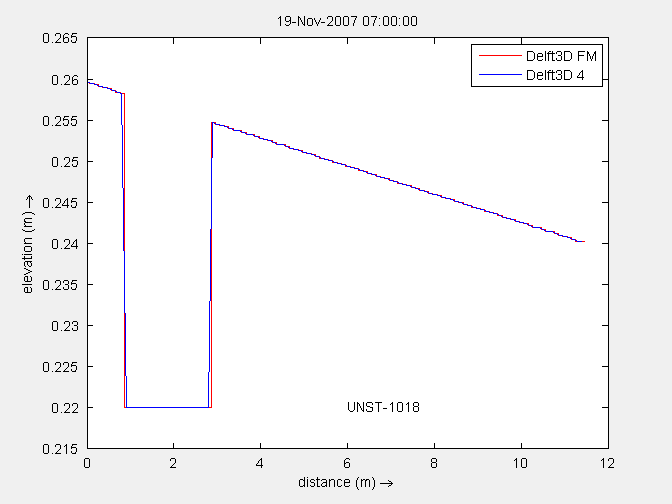
\includegraphics[width=0.70\textwidth]{figures/Delft3D_FM_vs_Delft3D_4.png}
	\end{center}
	\caption{Initial situation of the T2 experiment.}\label{fig:e02-fxx-cxx:initial}
\end{figure}

\paragraph*{Results}
The bed level after 2 and 4 hours are shown in Figure \ref{fig:e02-fxx-cxx:after2h} and Figure \ref{fig:e02-fxx-cxx:after4h}. Between 4 m and 7 meter a clear limiting of the erosion due to the lack of sediment is observed.

\begin{figure}[htb]
	\begin{center}
		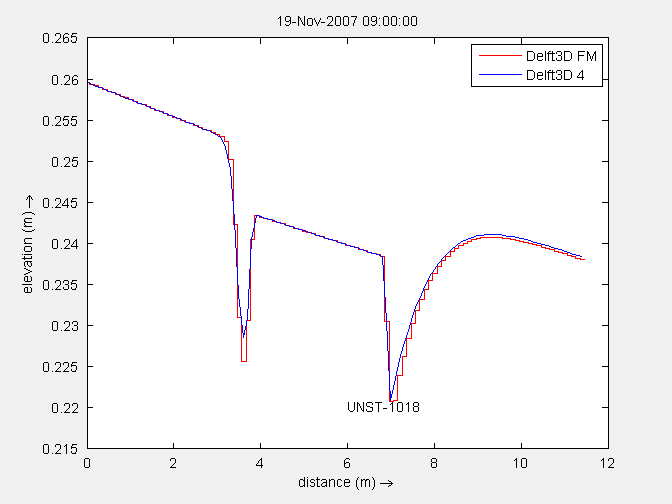
\includegraphics[width=0.70\textwidth]{figures/Delft3D_FM_vs_Delft3D_6.png}
	\end{center}
	\caption{Situation of the T2 experiment after 2 hours.}\label{fig:e02-fxx-cxx:after2h}
\end{figure}

\begin{figure}[htb]
	\begin{center}
		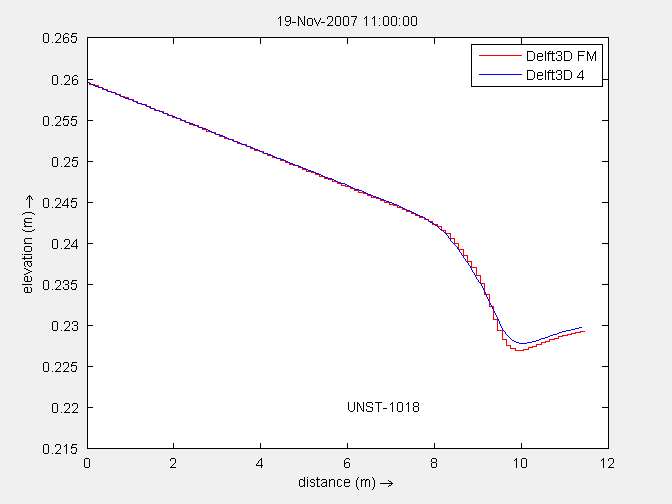
\includegraphics[width=0.70\textwidth]{figures/Delft3D_FM_vs_Delft3D_8.png}
	\end{center}
	\caption{Situation of the T2 experiment after 4 hours.}\label{fig:e02-fxx-cxx:after4h}
\end{figure}

\paragraph*{Conclusion}

The results indicate that Delft3D FM reproduces the result of Delft3D correctly.

\paragraph*{Version}
This test has been carried out with the following versions:
\begin{itemize}
\item Version 1.1.145.42461 of Delft3D FM.
\end{itemize}

\paragraph*{References}
\begin{thebibliography}{1}

\bibitem[{Gerritsen et~al.(2008)Gerritsen, De Goede, Platzek, Van Kester, Genseberger and Uittenbogaard}]{ValidationDocumentDelft3DFlow2008}
Gerriten, H., De Goede, E.D., Platzek, F.W., Van Kester, J.A.Th.M., Genseberger, M. and Uittenbogaard, R.E., 2008. Validation Document Delft3D-FLOW - A Software system for 3D flow simulations. Deltares, 182 pages.

\bibitem[{Struiksma (1999)}]{Struiksma1999}
Struiksma, N., 1999, Mathematical modelling of bedload transport over non-erodible layers. IAHR symposium on River, Coastal and Estuarine Morphodynamics (RCEM) Proceedings p.89-98. Genova.

\end{thebibliography}

\endinput
